\documentclass[stu,12pt,a4paper,floatsintext]{apa7}
\usepackage{graphicx}
\usepackage{float}
\usepackage{booktabs}
\usepackage{xcolor}
\usepackage{listings}
\usepackage{hyperref}

% Monospace listing style for depth maps
\lstset{
  basicstyle=\ttfamily\scriptsize,
  frame=single,
  backgroundcolor=\color[gray]{0.97},
  breaklines=false,
  columns=fixed,
  keepspaces=true,
}

\title{LLMs Mind's Eye: Text-Based Depth Representations as Spatial Reasoning Scaffolds}
\author{Robert Paszek}
\affiliation{Department of Cognitive Science and Artificial Intelligence, Tilburg University}
\course{Research Workshop}
\professor{Supervisor: Bruno Nicenboim}
\duedate{April 12, 2025}

\begin{document}
\maketitle

% ═══ PAGE 1: MOTIVATION + RQ ═══
\section*{Research Motivation}

Large language models (LLMs) have achieved remarkable performance across many reasoning tasks, yet they consistently fail at spatial reasoning. At launch of the ARC-AGI-2 benchmark, frontier models scored near 0\%, with only OpenAI's o3 reaching approximately 4\%, while humans averaged 75\% \cite{chollet2025}. Mental rotation tasks reduce multimodal LLMs to random chance---GPT-4o scores at or below the 32\% baseline \cite{stogiannidis2025}---and perspective-taking accuracy for GPT-4o from the human viewpoint is only 27.5\% compared to 99\% human performance \cite{shiri2024}. This gap persists despite massive increases in model scale, multimodal training, and chain-of-thought prompting.

From a societal perspective, spatial reasoning failures have real consequences: autonomous vehicle perception errors have caused fatal accidents when systems repeatedly misclassified pedestrians \cite{ntsb2019}, and of 49 FDA-cleared surgical robots, none operates above Level~3 autonomy \cite{lee2024}, due in part to the infancy of autonomous soft tissue manipulation \cite{khanna2025}. Scientifically, this failure is puzzling because LLMs excel at other forms of reasoning---mathematical proofs, code generation, logical deduction---but collapse when reasoning requires understanding 3D structure.

Current approaches to improving LLM spatial reasoning focus on adding vision modules: SpatialVLM embeds depth as features in vision-language models \cite{chen2024spatialvlm}, and DepthVLA adds depth streams to multimodal architectures \cite{yuan2025depthvla}. However, these approaches increase model complexity and remain tied to visual input. An alternative, under-explored hypothesis is that LLMs may already possess sufficient reasoning capability, but lack an appropriate \emph{representation format} for spatial information. Larkin and Simon~\cite{larkin1987} demonstrated formally that diagrams can make previously intractable problems trivially solvable---not by adding new information, but by making spatial relationships computationally accessible.

\section*{Research Question}

\begin{center}
\emph{To what extent do text-based depth representations, generated from a voxel domain-specific language, improve large language model performance on spatial reasoning tasks where current models score below 50\%?}
\end{center}

\section*{Background}

The theoretical foundation for this work comes from Larkin and Simon~\cite{larkin1987}, who proved that the computational difference between sentential and diagrammatic representations is not informational but structural: diagrams group spatially related information together, enabling perceptual operations that are computationally expensive in text. This principle suggests that converting spatial problems into structured, spatially-organized text could provide similar benefits for LLMs.

Recent work has begun exploring spatial intermediates for LLM reasoning. The Visualization-of-Thought (VoT) framework demonstrated that generating spatial intermediates (ASCII-like grids) during reasoning improved LLM performance on navigation and tiling tasks \cite{wu2024}. The Whiteboard-of-Thought (WoT) paradigm showed that a draw-render-perceive loop---where models generate visual code, render it, and interpret the output---improved spatial accuracy over pure text reasoning \cite{menon2024}. VoxPoser used LLMs to generate Python code that filled 3D voxel grids with affordance values for robot planning, achieving zero-shot generalization \cite{huang2023}.

However, no existing system implements a complete closed loop where an LLM writes 3D spatial code, receives text-based depth feedback from a raycasting camera system, verifies its reasoning against the rendered output, and iteratively revises---all without any vision model. The Mind's Eye system, which this proposal aims to evaluate, implements precisely this architecture using VOXI, a voxel description language, paired with a text-based raycaster that produces ASCII depth maps (digits 0--9 representing distance from camera). Figure~\ref{fig:feedback} shows the feedback mechanism.

% ═══ FIGURE 1: Compact 5-view pairs ═══
\begin{figure}[H]
\centering

% FRONT
\begin{minipage}[c]{0.28\textwidth}
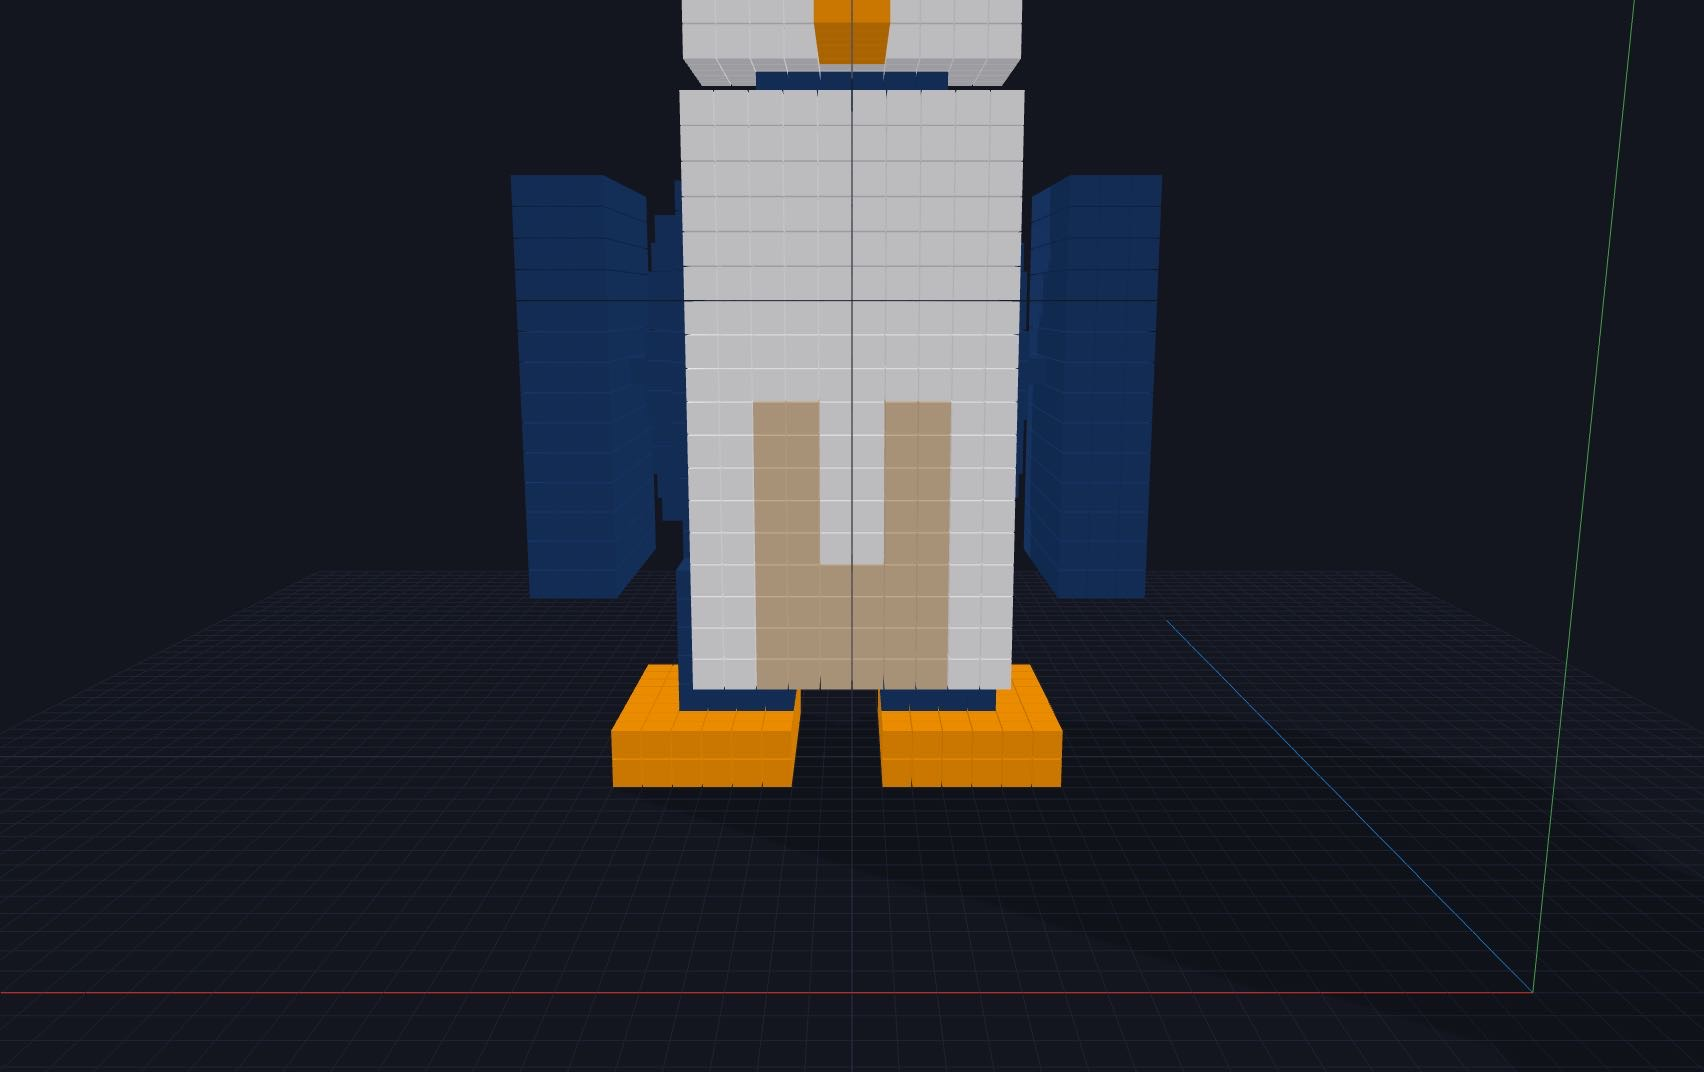
\includegraphics[width=\textwidth]{proposal-assets/penguin-render-front.jpg}
\end{minipage}%
\hfill
\begin{minipage}[c]{0.68\textwidth}
\begin{lstlisting}
FRONT (->X, ^Y) 32x32   .=empty 0=near 9=far
 0 . . . . . . . . . . . . 5 5 4 4 4 4 4 5 5 . . . . . . . . . . .
 3 . . . . . . . . . . . 3 3 3 2 2 2 2 3 3 3 5 . . . . . . . . . .
 9 . . . . . . . . . . . . . 4 4 4 4 4 4 6 . . . . . . . . . . . .
12 . . . . . . 4 4 4 . . 3 3 3 3 3 3 3 3 3 3 5 . . 4 4 4 . . . . .
18 . . . . . . 4 4 4 6 5 3 3 3 3 3 3 3 3 3 3 4 5 6 4 4 4 . . . . .
27 . . . . . . . . . . . 3 3 3 3 3 3 3 3 3 3 4 . . . . . . . . . .
31 . . . . . . . . . 4 4 4 4 4 4 . . . 4 4 4 4 4 4 . . . . . . . .
\end{lstlisting}
\end{minipage}

\vspace{6pt}

% RIGHT
\begin{minipage}[c]{0.28\textwidth}
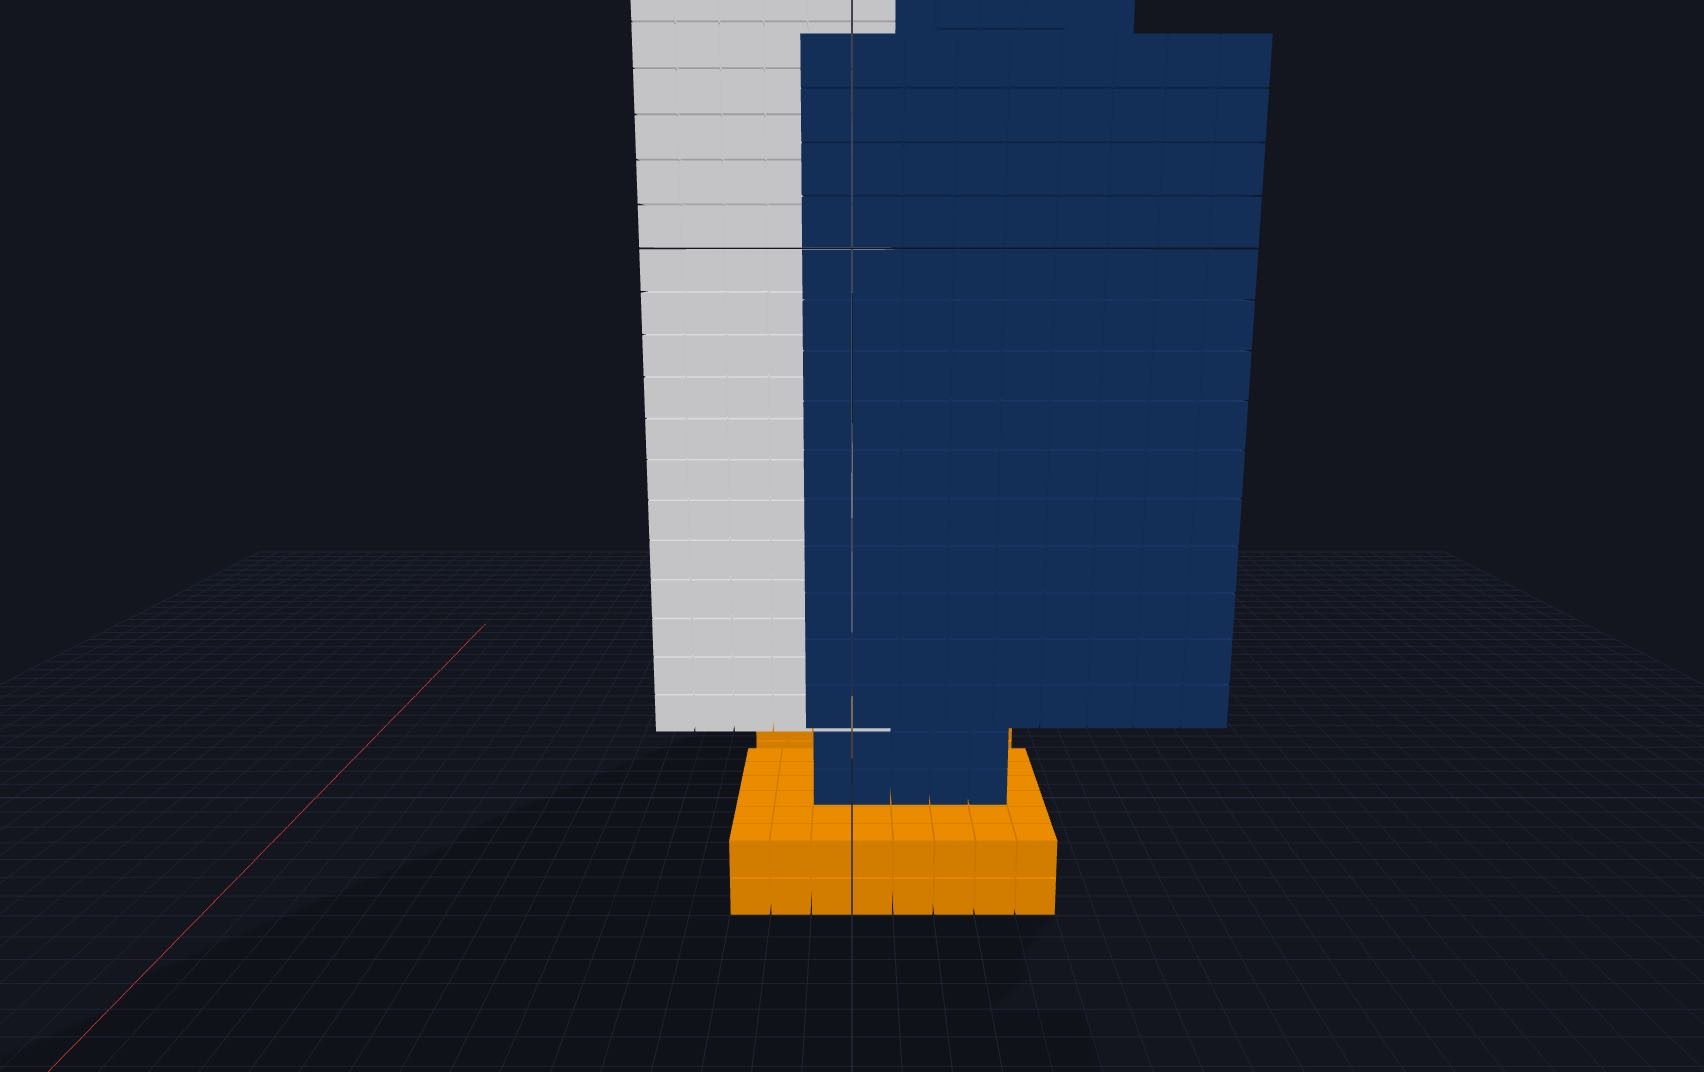
\includegraphics[width=\textwidth]{proposal-assets/penguin-render-right.jpg}
\end{minipage}%
\hfill
\begin{minipage}[c]{0.68\textwidth}
\begin{lstlisting}
RIGHT (->Z, ^Y) 32x32   .=empty 0=near 9=far
 0 . . . . . . . . . . . . . . 4 4 3 3 3 3 3 4 4 . . . . . . . . .
 9 . . . . . . . . . . . . . . 4 4 4 4 4 3 4 4 . . . . . . . . . .
12 . . . . . . . . . . . 3 3 3 3 1 1 1 1 1 1 1 1 1 . . . . . . . .
18 . . . . . . . . . . . 3 3 3 3 1 1 1 1 1 1 1 1 1 3 4 . . . . . .
27 . . . . . . . . . . . 3 3 3 3 3 3 3 3 3 4 4 . . . . . . . . . .
31 . . . . . . . . . . . . . 2 2 2 2 2 2 2 2 . . . . . . . . . . .
\end{lstlisting}
\end{minipage}

\vspace{6pt}

% BACK
\begin{minipage}[c]{0.28\textwidth}
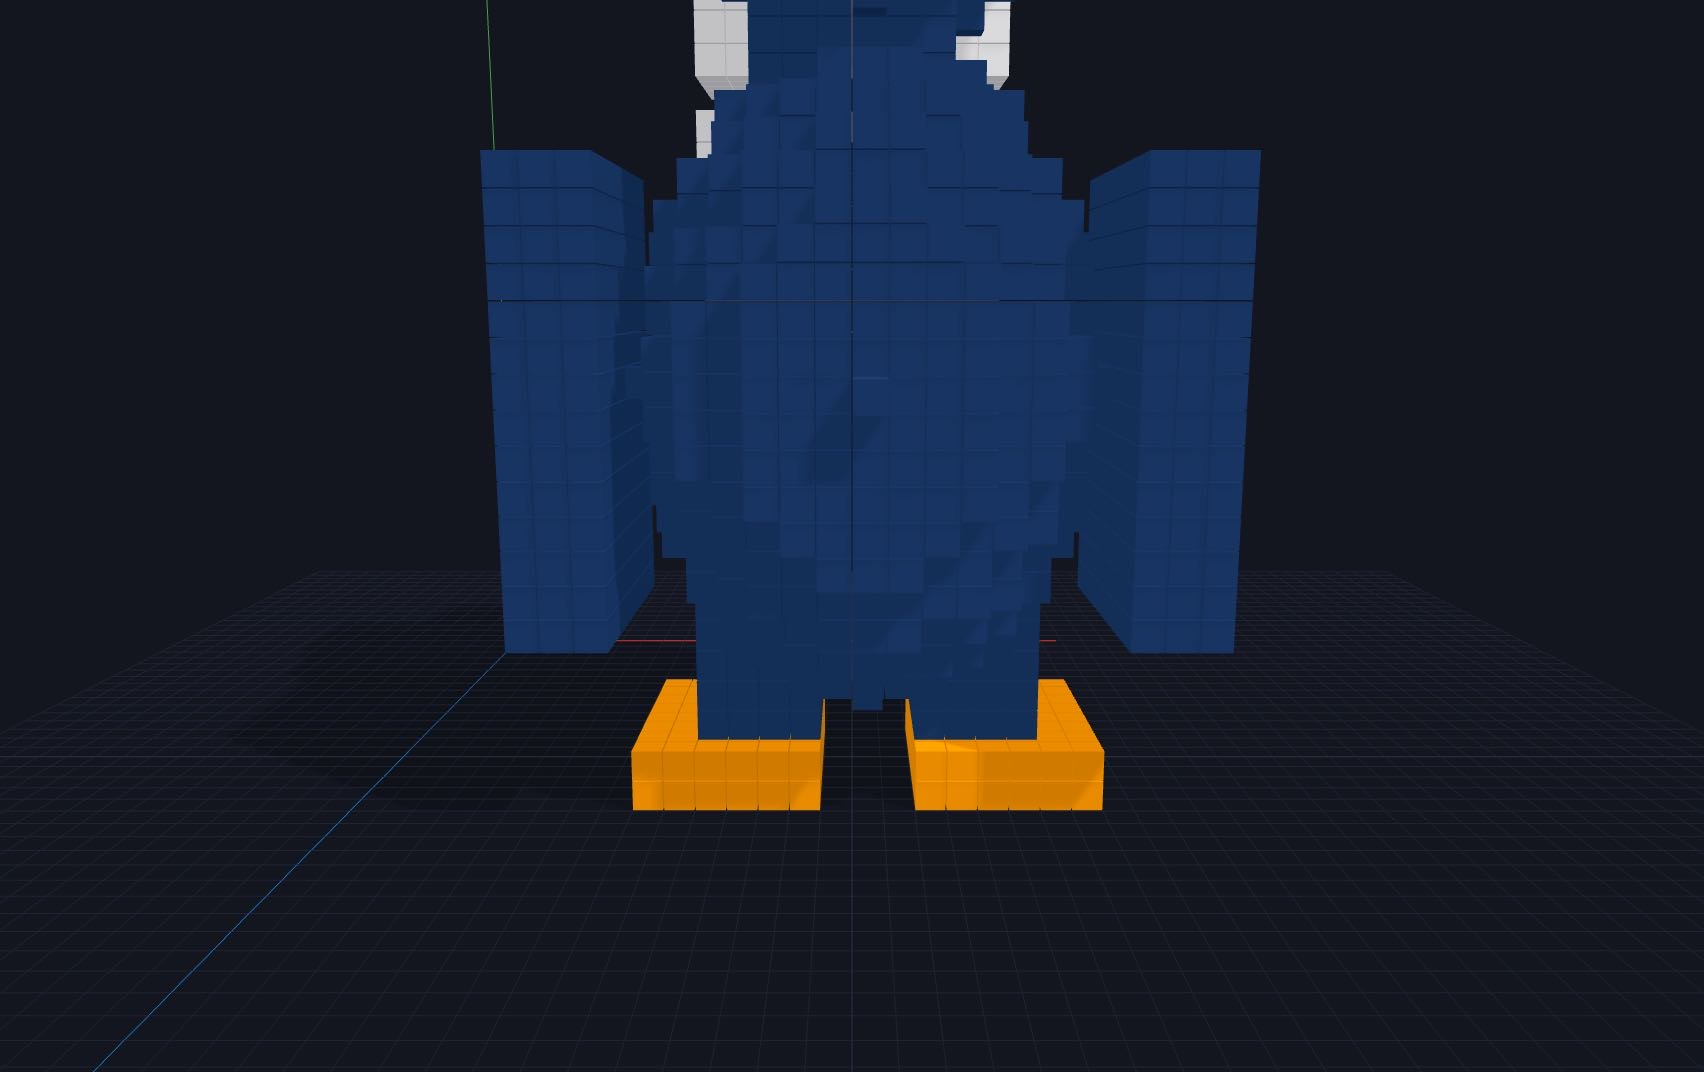
\includegraphics[width=\textwidth]{proposal-assets/penguin-render-back.jpg}
\end{minipage}%
\hfill
\begin{minipage}[c]{0.68\textwidth}
\begin{lstlisting}
BACK (->X, ^Y) 32x32    .=empty 0=near 9=far
 0 . . . . . . . . . . . 4 3 3 3 3 3 3 3 4 . . . . . . . . . . . .
 9 . . . . . . . . . . . . 3 3 3 3 3 3 3 . . . . . . . . . . . . .
12 . . . . . 2 2 2 . . 3 3 2 2 2 2 2 2 2 3 3 . . 2 2 2 . . . . . .
18 . . . . . 2 2 2 3 3 2 2 2 2 2 2 2 2 2 2 2 3 3 2 2 2 . . . . . .
27 . . . . . . . . . . 3 3 3 3 3 3 3 3 3 3 3 . . . . . . . . . . .
31 . . . . . . . . 3 3 3 3 3 3 . . . 3 3 3 3 3 3 . . . . . . . . .
\end{lstlisting}
\end{minipage}

\vspace{6pt}

% LEFT
\begin{minipage}[c]{0.28\textwidth}
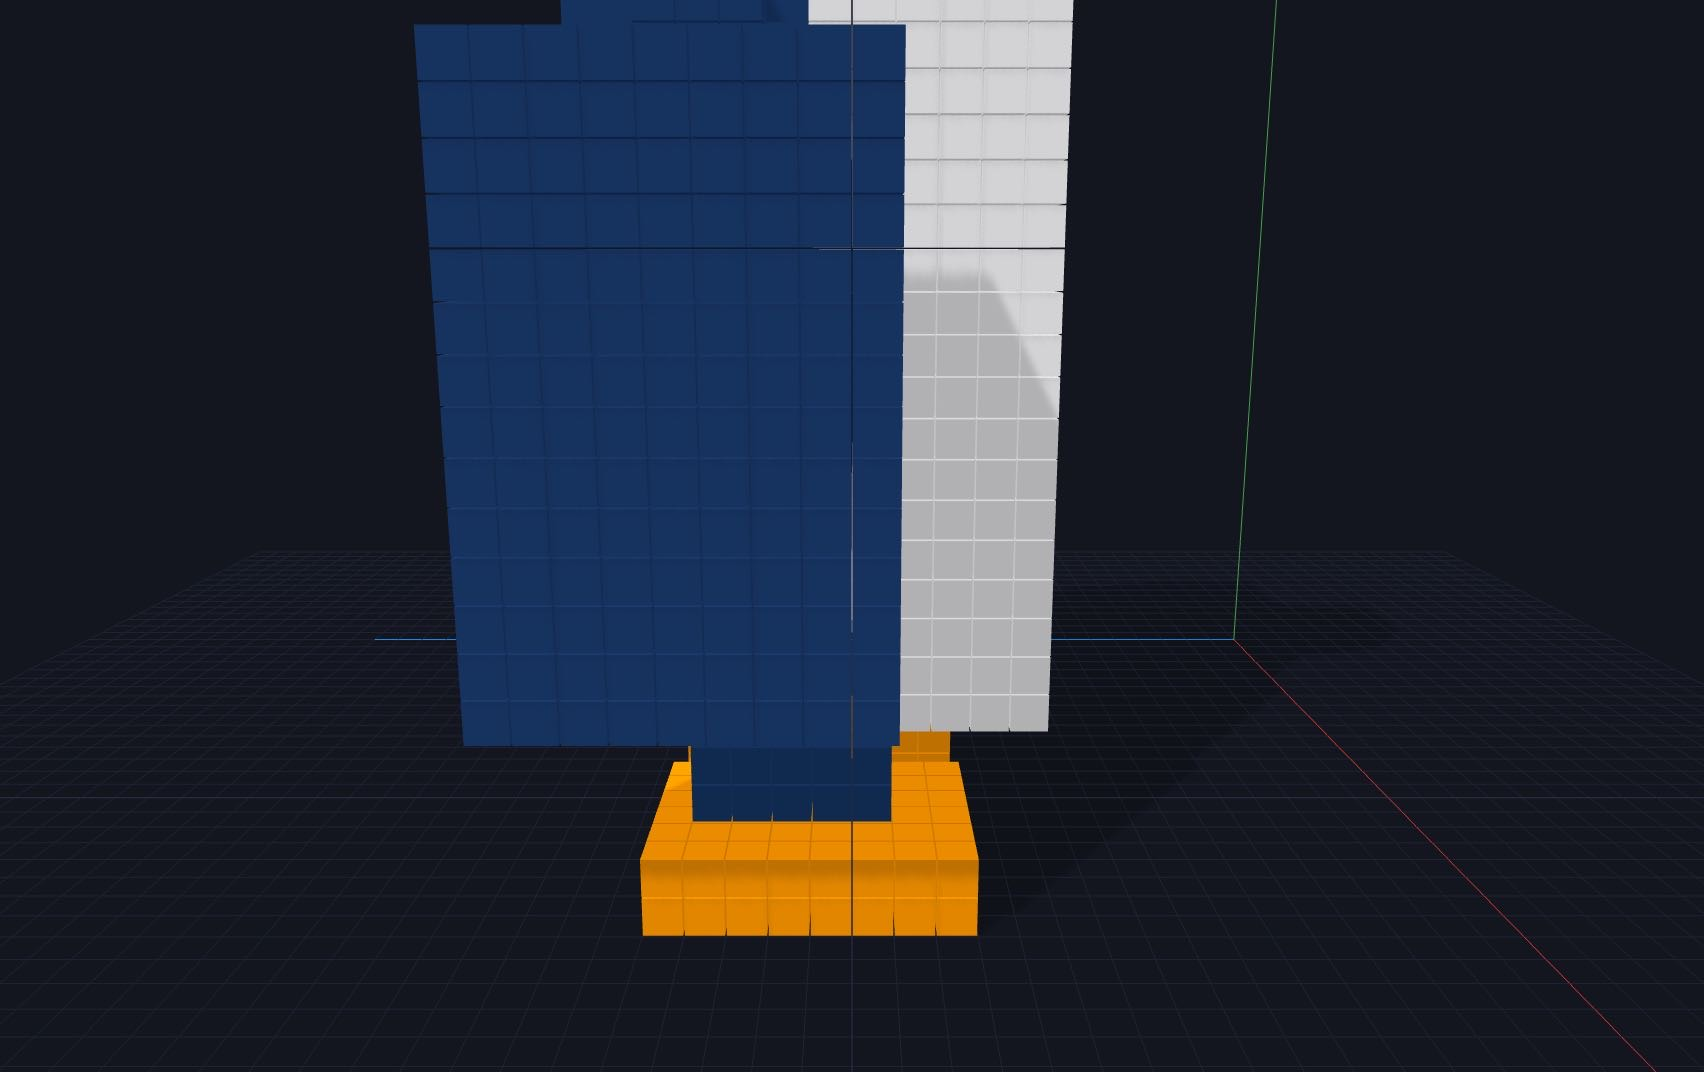
\includegraphics[width=\textwidth]{proposal-assets/penguin-render-left.jpg}
\end{minipage}%
\hfill
\begin{minipage}[c]{0.68\textwidth}
\begin{lstlisting}
LEFT (->Z, ^Y) 32x32    .=empty 0=near 9=far
 0 . . . . . . . . . 5 4 4 4 3 4 4 4 5 . . . . . . . . . . . . . .
 9 . . . . . . . . . . 4 4 4 4 4 4 4 4 . . . . . . . . . . . . . .
12 . . . . . . . . 2 2 2 2 2 2 2 2 2 3 3 3 3 . . . . . . . . . . .
18 . . . . . . 5 4 2 2 2 2 2 2 2 2 2 3 3 3 3 . . . . . . . . . . .
27 . . . . . . . . . . 4 4 3 3 3 3 3 3 3 3 3 . . . . . . . . . . .
31 . . . . . . . . . . . 3 3 3 3 3 3 3 3 . . . . . . . . . . . . .
\end{lstlisting}
\end{minipage}

\vspace{6pt}

% TOP
\begin{minipage}[c]{0.28\textwidth}
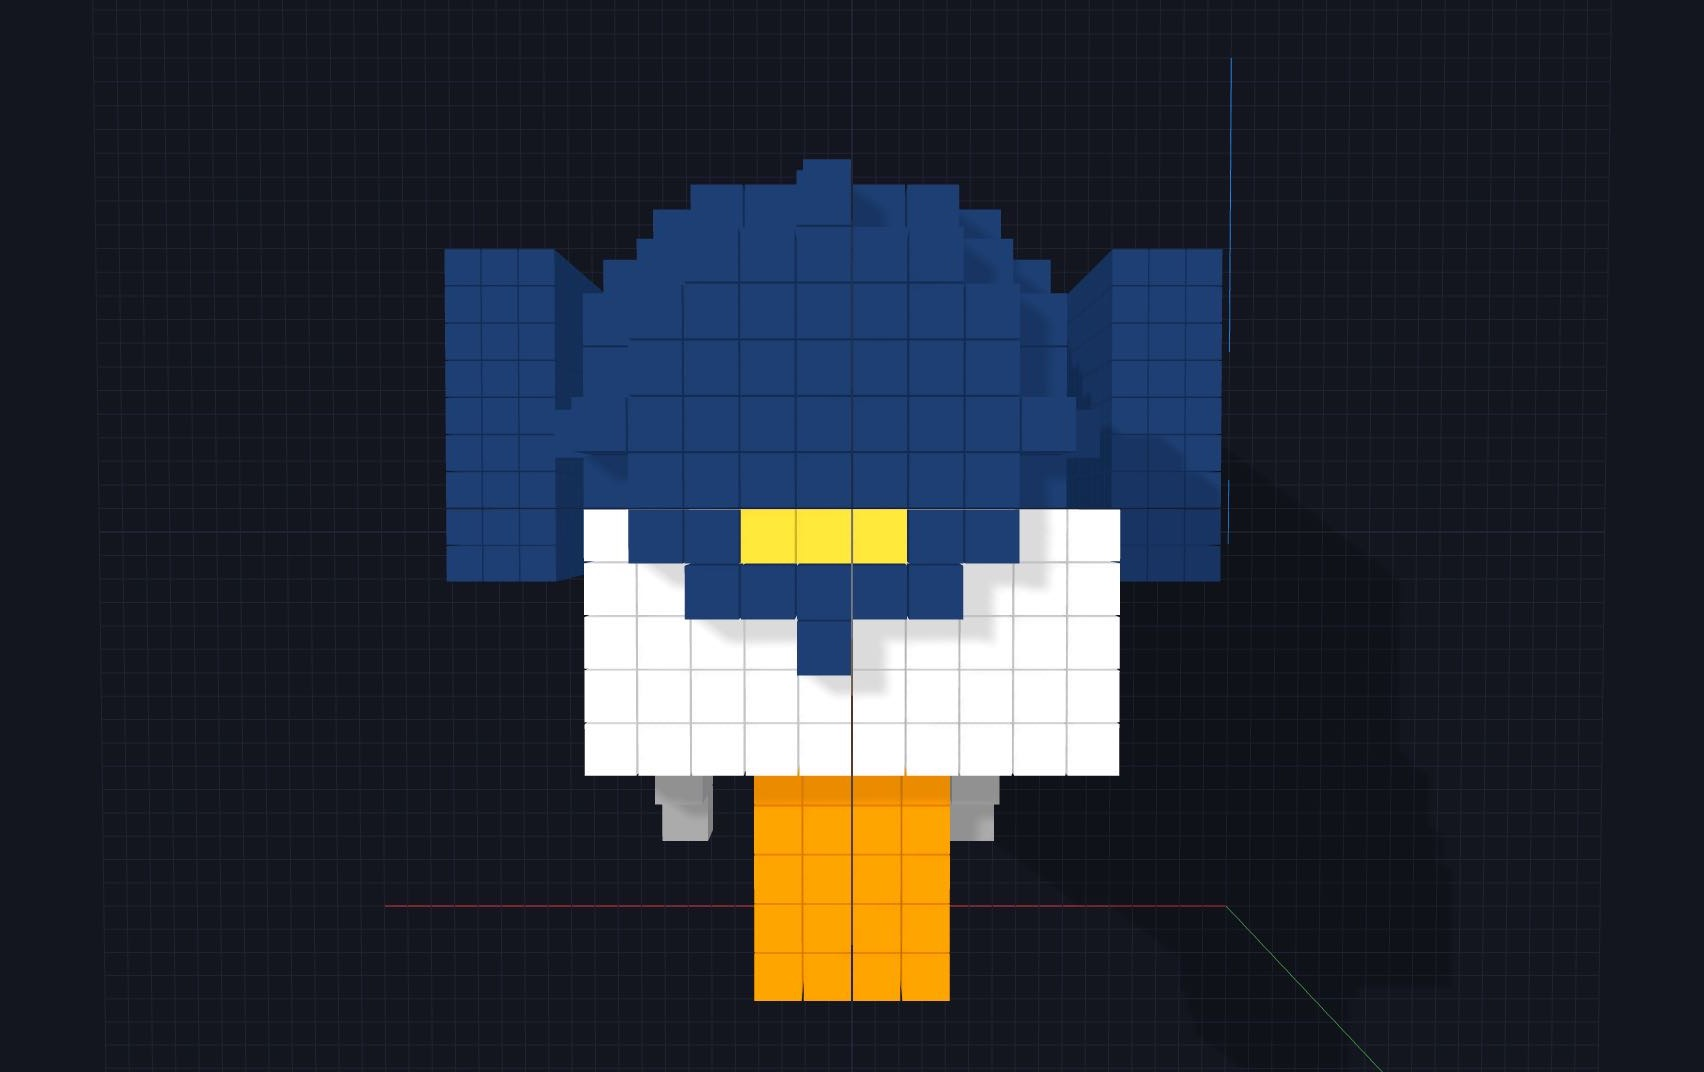
\includegraphics[width=\textwidth]{proposal-assets/penguin-render-top.jpg}
\end{minipage}%
\hfill
\begin{minipage}[c]{0.68\textwidth}
\begin{lstlisting}
TOP (->X, ^Z) 32x32     .=empty 0=near 9=far
 8 . . . . . . 3 3 3 . . 5 4 3 3 3 1 3 3 3 4 5 . . 3 3 3 . . . . .
 9 . . . . . . 3 3 3 . 5 4 3 1 0 0 0 0 0 1 3 4 5 . 3 3 3 . . . . .
11 . . . . . . 3 3 3 9 4 3 0 0 0 0 0 0 0 0 0 3 4 9 3 3 3 . . . . .
17 . . . . . . . . . 9 9 0 0 0 0 0 0 0 0 0 0 9 9 9 . . . . . . . .
19 . . . . . . . . . . . 0 0 0 0 0 0 0 0 0 0 . . . . . . . . . . .
21 . . . . . . . . . . . . . 1 1 1 1 1 . 1 . . . . . . . . . . . .
\end{lstlisting}
\end{minipage}

\caption{The Mind's Eye feedback mechanism applied to a voxel penguin (32$\times$32$\times$32). Left column: 3D WebGL renders from five orthographic cameras. Right column: the corresponding text-based depth maps the LLM reads. Each digit (0--9) encodes ray-traced distance from the virtual camera. The LLM receives only the text---no vision model is involved. Full-resolution maps in the Appendix.}
\label{fig:feedback}
\end{figure}

% ═══ PAGE 3: METHODS ═══
\section*{Methods}

\subsection*{Experimental Design}

This study employs a 2$\times$2 factorial design with two independent variables: (a) \emph{representation type} (natural language only vs.\ natural language augmented with text-based depth matrices) and (b) \emph{model capability level} (high-capability model: Claude Sonnet vs.\ lower-capability model: Claude Haiku). The dependent variable is task accuracy (percentage of correctly answered spatial reasoning questions).

\subsection*{Datasets}

Three existing benchmarks will be used. First, the SpartQA dataset \cite{mirzaee2021}, consisting of multi-hop spatial reasoning questions derived from natural language scene descriptions (e.g., ``What is the relation of block A to block C?'' requiring transitive inference through block B). Twenty tasks of varying difficulty will be sampled. Second, the CATER video benchmark \cite{girdhar2020}, providing real-world video scenes requiring 3D spatial understanding; five tasks involving object counting, motion tracking, and occlusion detection will be used, with depth matrices extracted at 20$\times$20 resolution using Depth Anything V2. Third, thirty automatically generated VOXI scenes (16$\times$16$\times$16 grids, seed=42) with five question types: collision detection, relative position, motion direction, object count, and closer-to-camera judgments.

\subsection*{Feature Extraction}

For the depth-matrix condition, the Mind's Eye system converts spatial information into structured text through orthographic raycasting. For each scene, six depth maps (front, back, left, right, top, bottom) are generated as character grids where each cell contains a digit 0--9 representing normalized depth. For CATER video, monocular depth estimation (Depth Anything V2) produces per-frame 20$\times$20 depth matrices quantized to the same 0--9 range. The control condition receives only the original natural language descriptions or VOXI source code without depth rendering.

\subsection*{Procedure}

Each model-condition combination will be tested on all tasks. For each task, the LLM receives the spatial problem description and (in the depth condition) the corresponding depth matrices. The model produces an answer, which is compared against the ground truth. No iterative refinement is permitted during benchmarking---each answer must be given in a single pass to ensure controlled comparison.

\subsection*{Statistical Analysis}

A two-way analysis of variance (ANOVA) will test the main effects of representation type and model capability, as well as their interaction. Given preliminary results suggesting that the tool helps high-capability models but may hurt lower-capability ones, the interaction effect is of particular theoretical interest. Post-hoc comparisons using Tukey's HSD will identify significant pairwise differences. Additionally, accuracy will be broken down by task type (collision, position, motion, count, occlusion) to identify which spatial reasoning subtasks benefit most from depth representations. Effect sizes (Cohen's \emph{d}) will be reported for all significant comparisons.

% ═══ REFERENCES ═══
\newpage
\begin{thebibliography}{9}

\bibitem[Chen et al., 2024]{chen2024spatialvlm}
Chen, B., Xu, Z., Kirmani, S., Ichter, B., Driess, D., Florence, P., Sadigh, D., Guibas, L., \& Xia, F. (2024). SpatialVLM: Endowing vision-language models with spatial reasoning capabilities. \emph{Proceedings of the IEEE/CVF Conference on Computer Vision and Pattern Recognition (CVPR)}.

\bibitem[Chollet et al., 2025]{chollet2025}
Chollet, F., Knoop, M., Kamradt, G., Landers, B., \& Pinkard, H. (2025). ARC-AGI-2: A new challenge for frontier AI reasoning systems. \emph{arXiv preprint arXiv:2505.11831}.

\bibitem[Girdhar \& Ramanan, 2020]{girdhar2020}
Girdhar, R., \& Ramanan, D. (2020). CATER: A diagnostic dataset for compositional actions and temporal reasoning. \emph{International Conference on Learning Representations}.

\bibitem[Huang et al., 2023]{huang2023}
Huang, W., Wang, C., Zhang, R., Li, Y., Wu, J., \& Fei-Fei, L. (2023). VoxPoser: Composable 3D value maps for robotic manipulation with language models. \emph{Conference on Robot Learning}.

\bibitem[Larkin \& Simon, 1987]{larkin1987}
Larkin, J. H., \& Simon, H. A. (1987). Why a diagram is (sometimes) worth ten thousand words. \emph{Cognitive Science, 11}(1), 65--100. \url{https://doi.org/10.1111/j.1551-6708.1987.tb00863.x}

\bibitem[Mirzaee et al., 2021]{mirzaee2021}
Mirzaee, R., Faghihi, H. R., Ning, Q., \& Kordjamshidi, P. (2021). SpartQA: A textual question answering benchmark for spatial reasoning. \emph{Findings of the Association for Computational Linguistics: ACL-IJCNLP 2021}.

\bibitem[Khanna et al., 2025]{khanna2025}
Khanna, R., Raison, N., Granados Martinez, A., Ourselin, S., Montorsi, F., Briganti, A., \& Dasgupta, P. (2025). At the cutting edge: The potential of autonomous surgery and challenges faced. \emph{BMJ Surgery, Interventions, \& Health Technologies, 7}(1), e000338. \url{https://doi.org/10.1136/bmjsit-2024-000338}

\bibitem[Lee et al., 2024]{lee2024}
Lee, A., Baker, T. S., Bederson, J. B., \& Rapoport, B. I. (2024). Levels of autonomy in FDA-cleared surgical robots: A systematic review. \emph{npj Digital Medicine, 7}, 103. \url{https://doi.org/10.1038/s41746-024-01102-y}

\bibitem[Menon et al., 2024]{menon2024}
Menon, S., Zemel, R., \& Vondrick, C. (2024). Whiteboard-of-thought: Thinking step-by-step across modalities. \emph{arXiv preprint arXiv:2406.14562}.

\bibitem[{National Transportation Safety Board}, 2019]{ntsb2019}
{National Transportation Safety Board}. (2019). \emph{Collision between vehicle controlled by developmental automated driving system and pedestrian, Tempe, Arizona, March 18, 2018} (Highway Accident Report NTSB/HAR-19/03). Washington, DC.

\bibitem[Shiri et al., 2024]{shiri2024}
Shiri, F., Guo, X.-Y., Far, M. G., Yu, X., Haffari, G., \& Li, Y.-F. (2024). An empirical analysis on spatial reasoning capabilities of large multimodal models. \emph{Proceedings of the 2024 Conference on Empirical Methods in Natural Language Processing (EMNLP)}.

\bibitem[Stogiannidis et al., 2025]{stogiannidis2025}
Stogiannidis, I., McDonagh, S., \& Tsaftaris, S. A. (2025). Mind the gap: Benchmarking spatial reasoning in vision-language models. \emph{arXiv preprint arXiv:2503.19707}.

\bibitem[Wu et al., 2024]{wu2024}
Wu, W., Mao, S., Zhang, Y., Xia, Y., Dong, L., Cui, L., \& Wei, F. (2024). Visualization-of-thought elicits spatial reasoning in large language models. \emph{arXiv preprint arXiv:2404.03622}.

\bibitem[Yuan et al., 2025]{yuan2025depthvla}
Yuan, T., Liu, Y., Lu, C., Chen, Z., Jiang, T., \& Zhao, H. (2025). DepthVLA: Enhancing vision-language-action models with depth-aware spatial reasoning. \emph{arXiv preprint arXiv:2510.13375}.

\end{thebibliography}

% ═══ APPENDIX ═══
\newpage
\begin{center}
{\large\bfseries Appendix: Full-Resolution Mind's Eye Depth Maps}\\[6pt]
\normalsize Voxel Penguin Model (32$\times$32$\times$32) --- 5 Orthographic Views\\
Left: 3D WebGL render. Right: text-based depth map (what the LLM reads).\\
\textbf{No vision model is used. The LLM receives only the text.}\\[6pt]
\small\textbf{Depth encoding:} \texttt{.} = empty \quad \texttt{0} = closest to camera \quad \texttt{1--8} = progressively deeper \quad \texttt{9} = farthest
\end{center}

\vspace{12pt}

% FRONT
\noindent\textbf{FRONT View}\\[-4pt]
\rule{\textwidth}{0.4pt}

\noindent
\begin{minipage}[t]{0.45\textwidth}
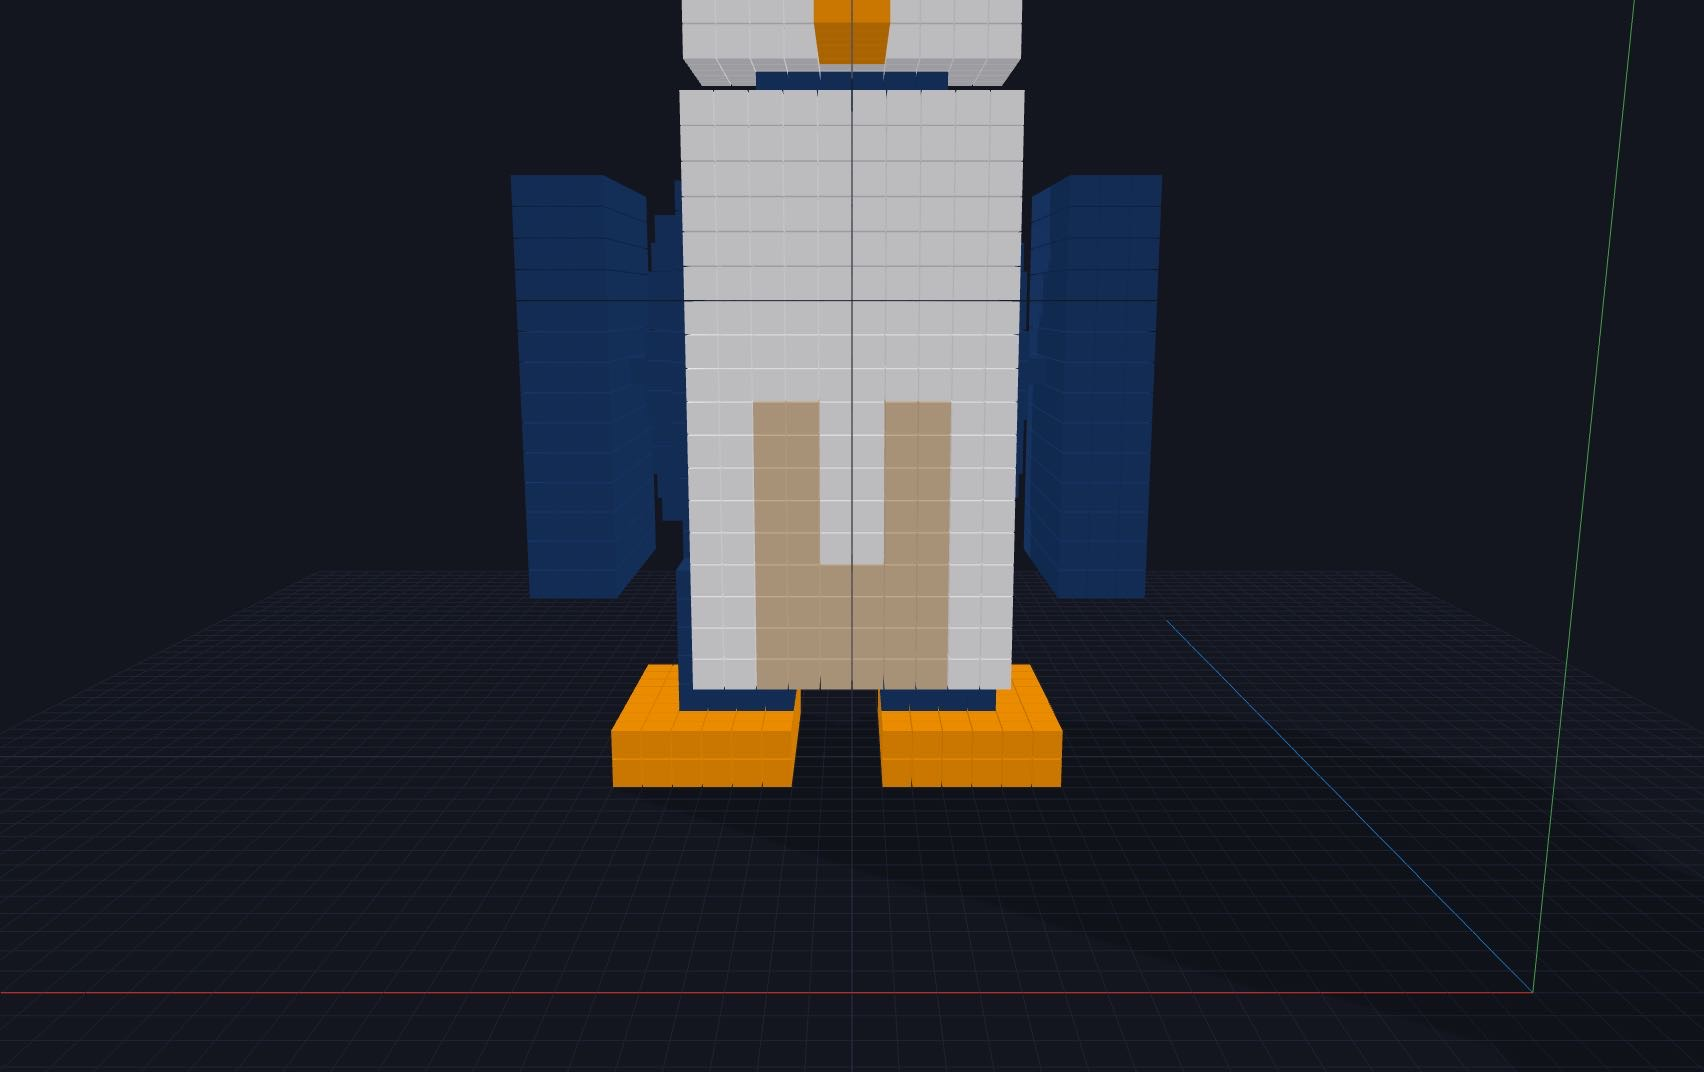
\includegraphics[width=\textwidth]{proposal-assets/penguin-render-front.jpg}
\end{minipage}%
\hfill
\begin{minipage}[t]{0.52\textwidth}
\lstinputlisting[basicstyle=\ttfamily\fontsize{5}{6}\selectfont]{proposal-assets/penguin-full-front.txt}
\end{minipage}

\vspace{8pt}

% RIGHT
\noindent\textbf{RIGHT View}\\[-4pt]
\rule{\textwidth}{0.4pt}

\noindent
\begin{minipage}[t]{0.45\textwidth}
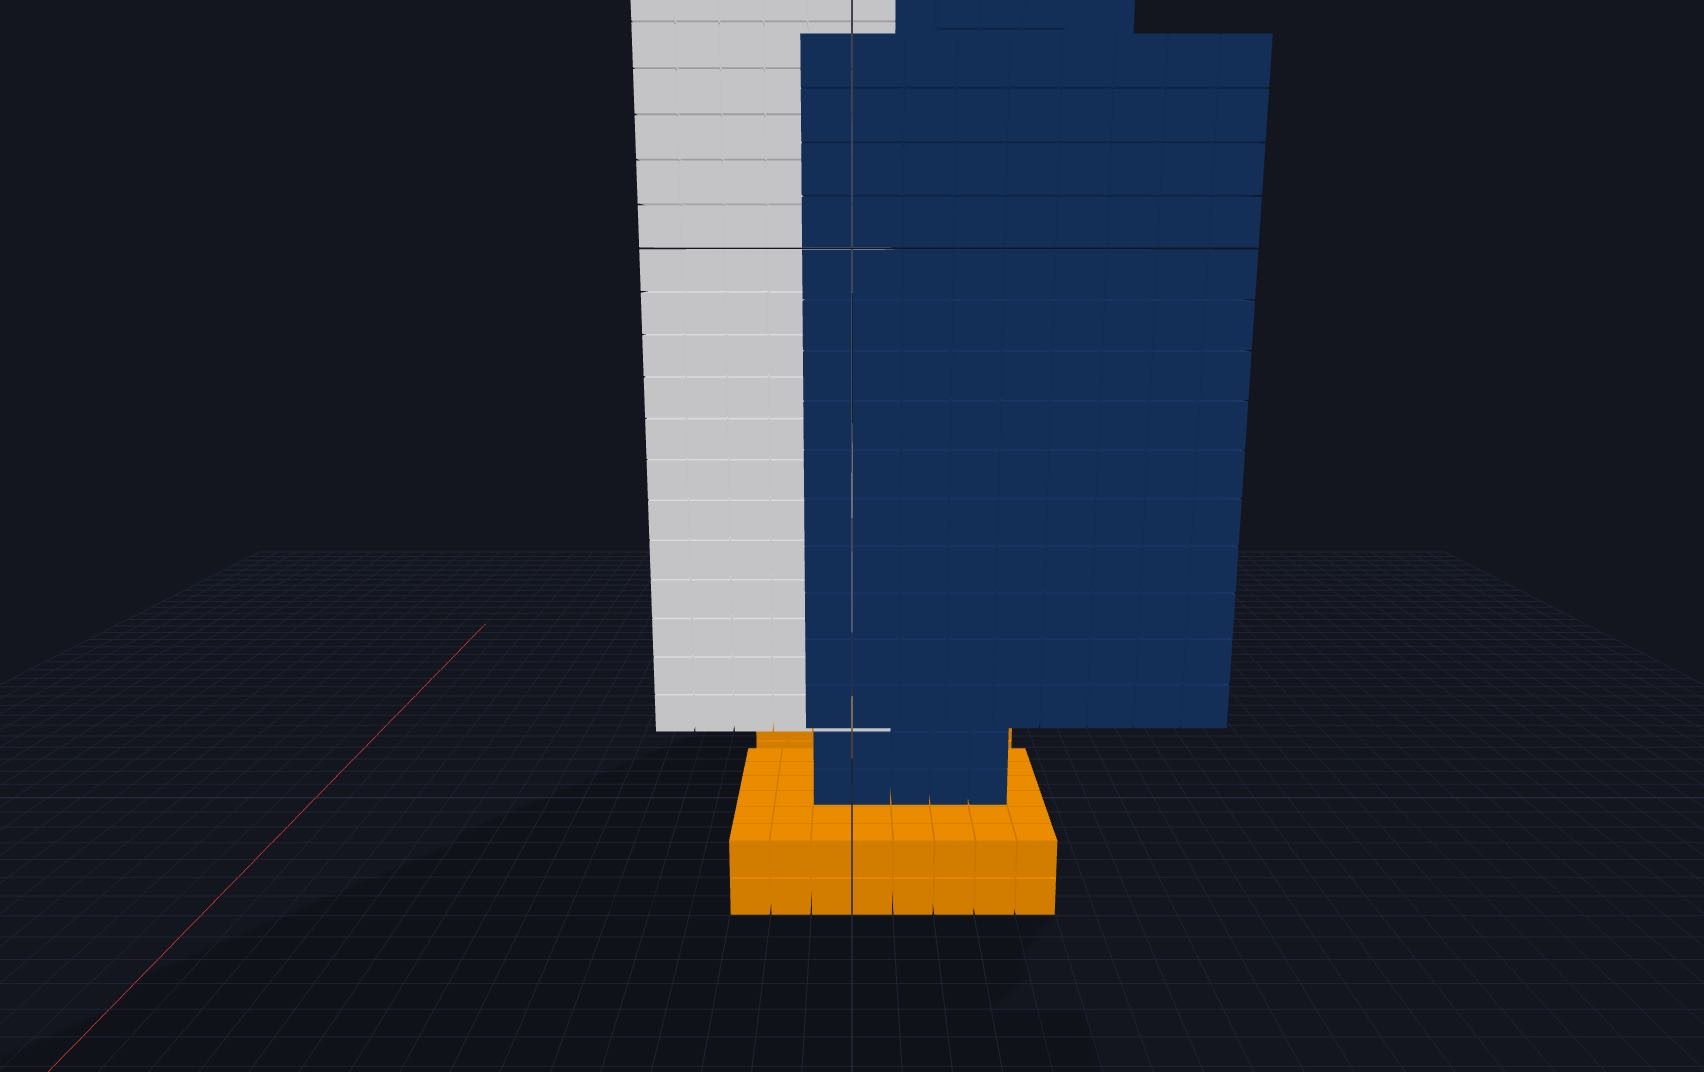
\includegraphics[width=\textwidth]{proposal-assets/penguin-render-right.jpg}
\end{minipage}%
\hfill
\begin{minipage}[t]{0.52\textwidth}
\lstinputlisting[basicstyle=\ttfamily\fontsize{5}{6}\selectfont]{proposal-assets/penguin-full-right.txt}
\end{minipage}

\vspace{8pt}

% BACK
\noindent\textbf{BACK View}\\[-4pt]
\rule{\textwidth}{0.4pt}

\noindent
\begin{minipage}[t]{0.45\textwidth}
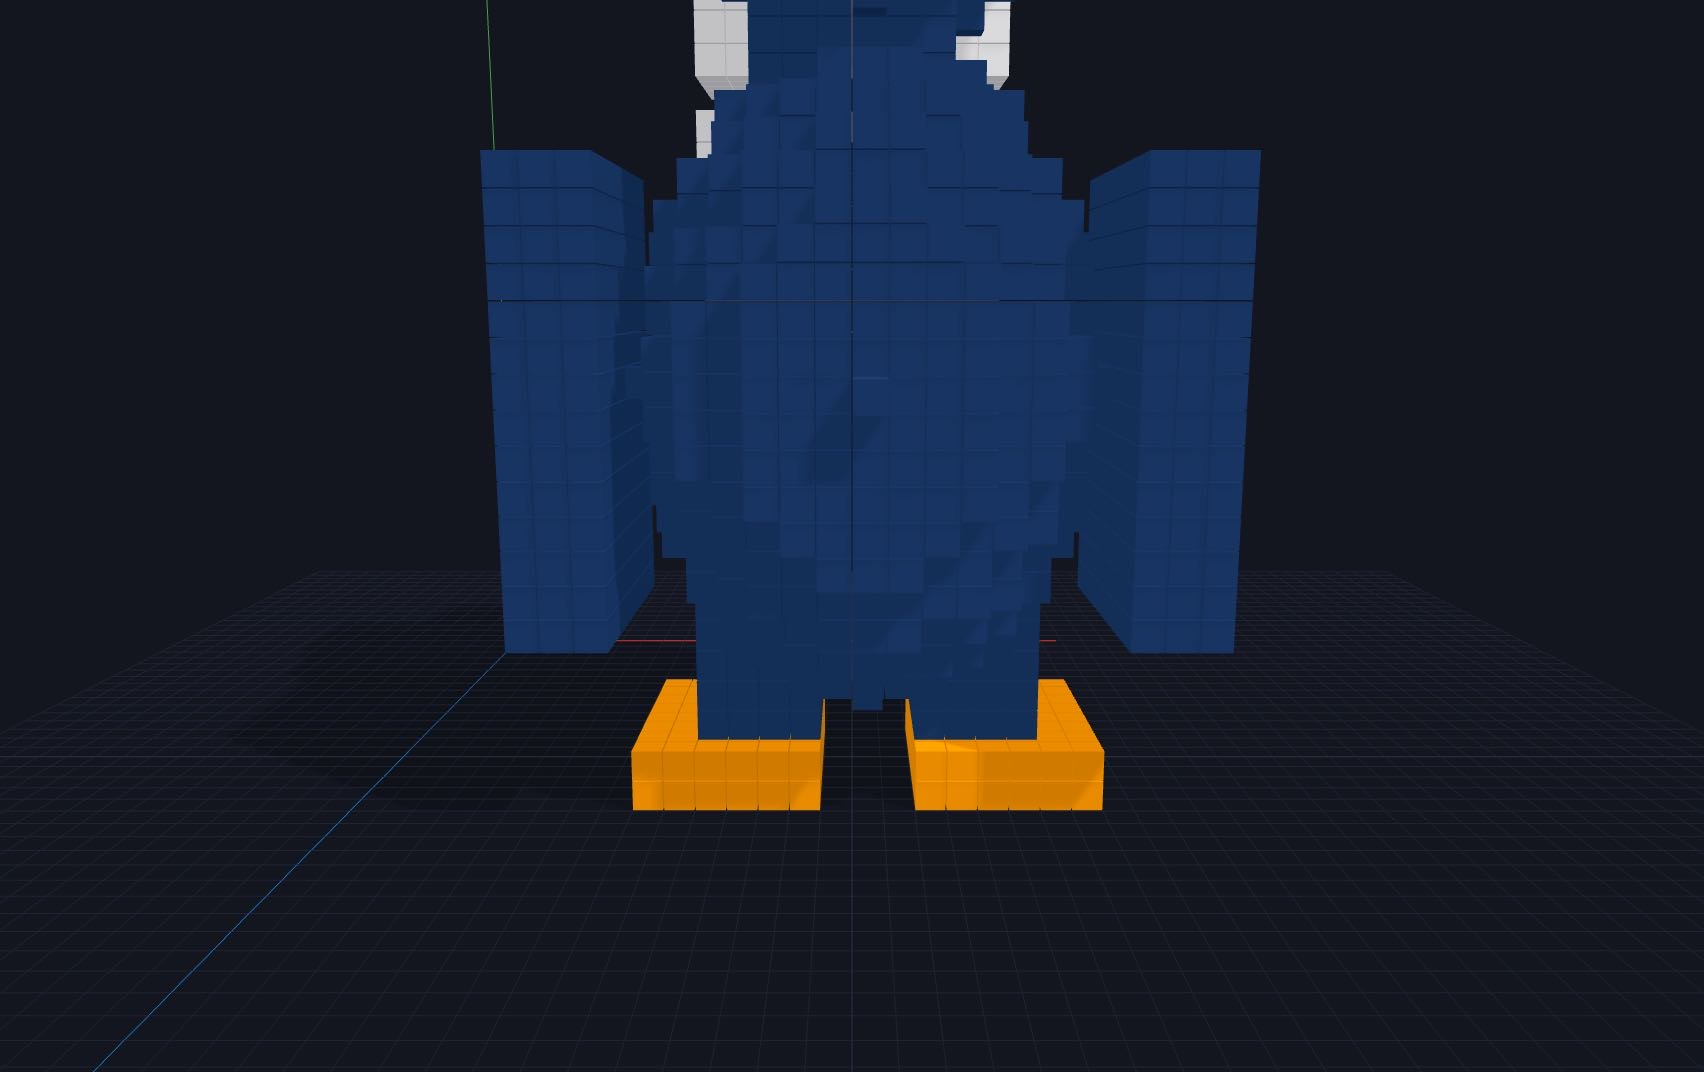
\includegraphics[width=\textwidth]{proposal-assets/penguin-render-back.jpg}
\end{minipage}%
\hfill
\begin{minipage}[t]{0.52\textwidth}
\lstinputlisting[basicstyle=\ttfamily\fontsize{5}{6}\selectfont]{proposal-assets/penguin-full-back.txt}
\end{minipage}

\newpage

% LEFT
\noindent\textbf{LEFT View}\\[-4pt]
\rule{\textwidth}{0.4pt}

\noindent
\begin{minipage}[t]{0.45\textwidth}
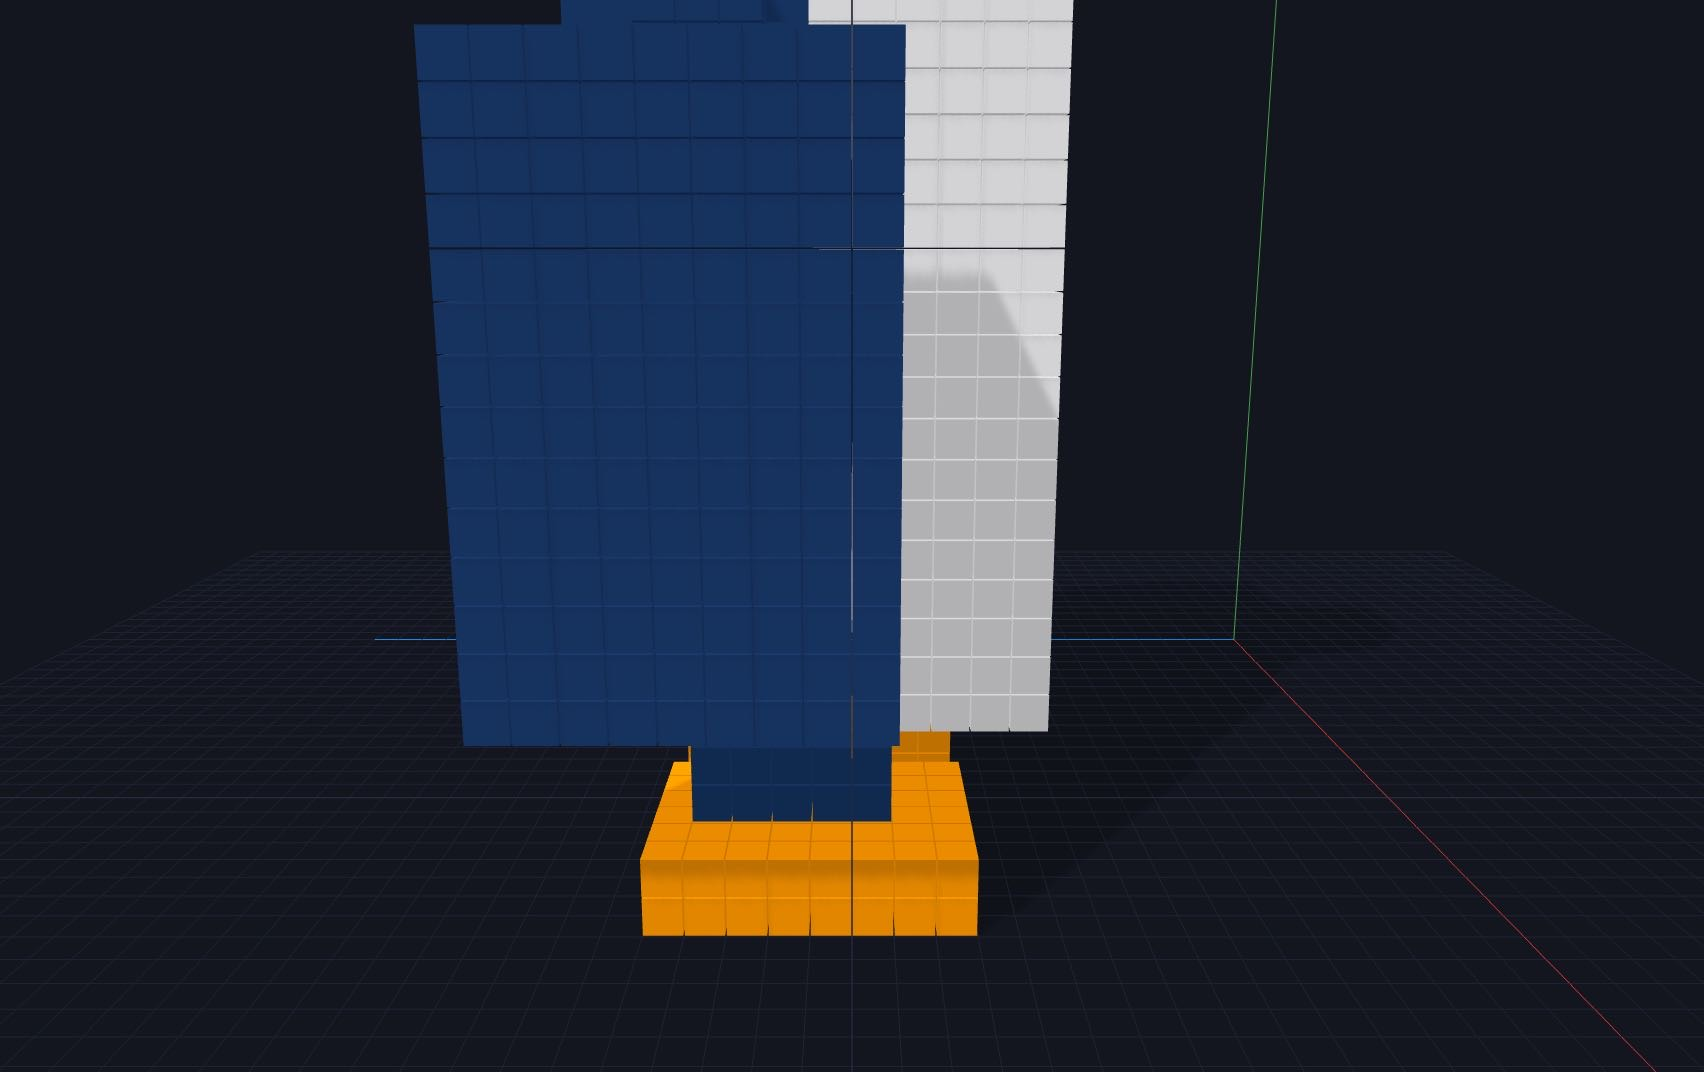
\includegraphics[width=\textwidth]{proposal-assets/penguin-render-left.jpg}
\end{minipage}%
\hfill
\begin{minipage}[t]{0.52\textwidth}
\lstinputlisting[basicstyle=\ttfamily\fontsize{5}{6}\selectfont]{proposal-assets/penguin-full-left.txt}
\end{minipage}

\vspace{8pt}

% TOP
\noindent\textbf{TOP View}\\[-4pt]
\rule{\textwidth}{0.4pt}

\noindent
\begin{minipage}[t]{0.45\textwidth}
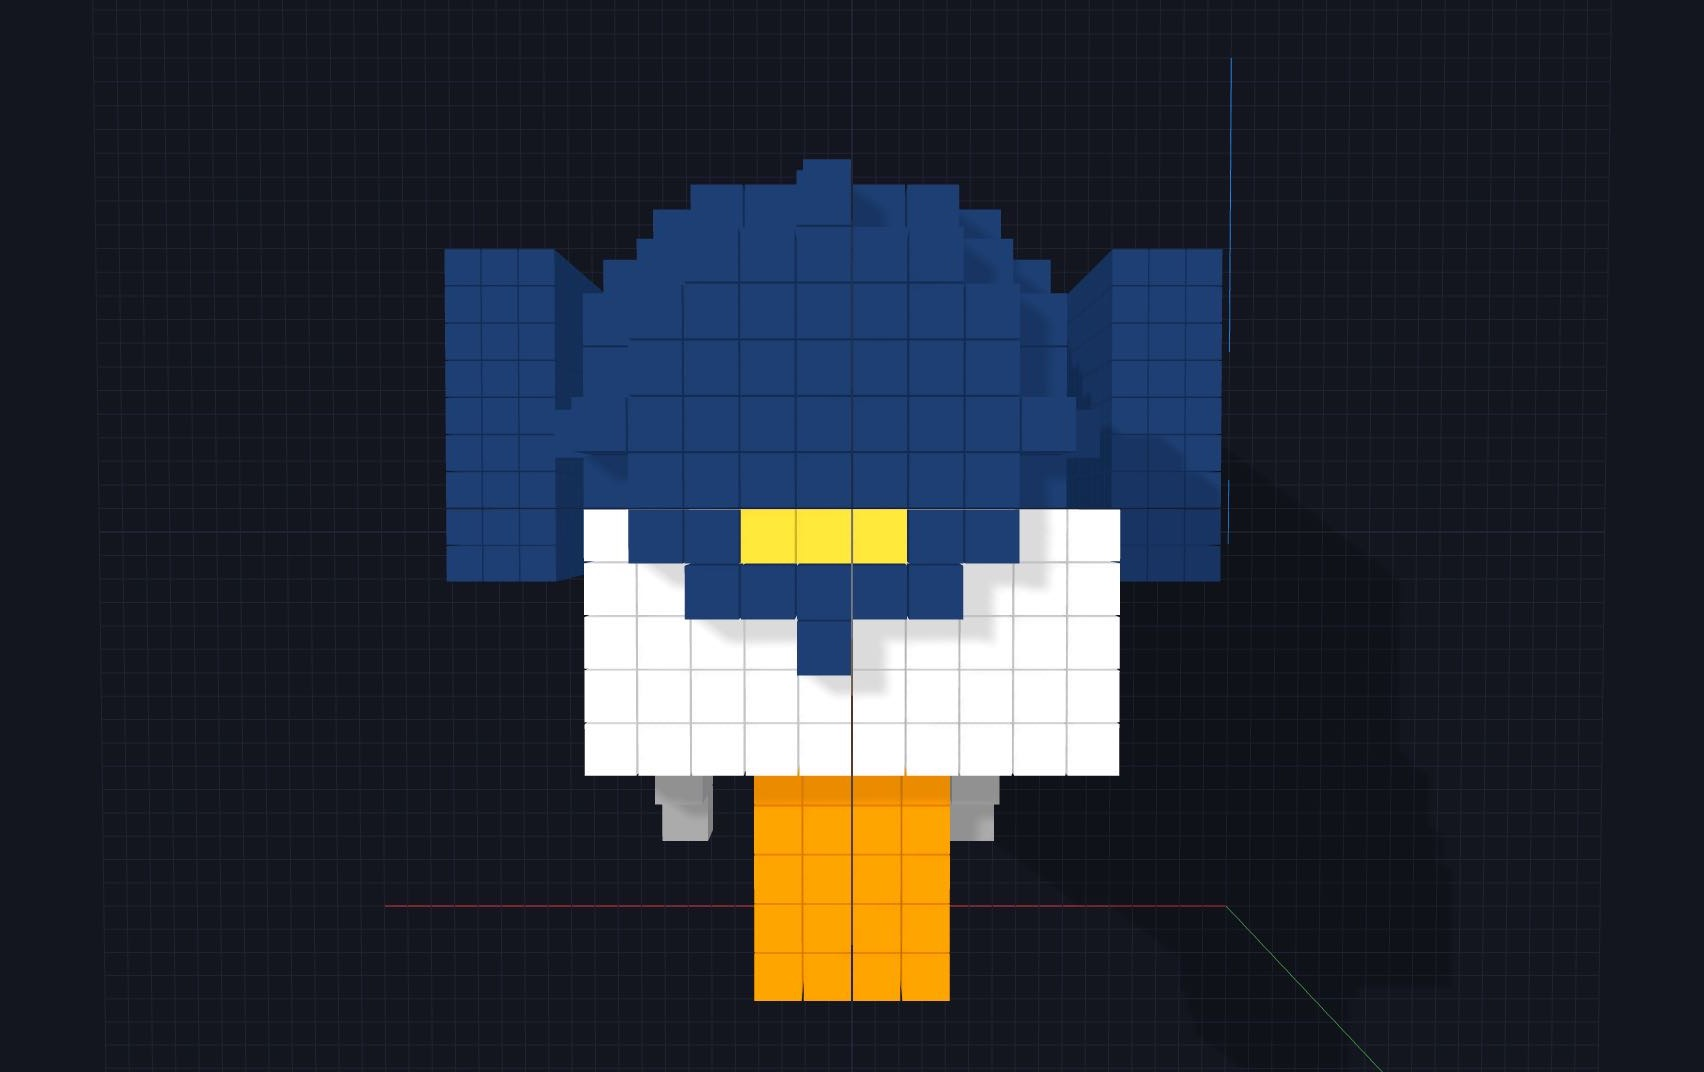
\includegraphics[width=\textwidth]{proposal-assets/penguin-render-top.jpg}
\end{minipage}%
\hfill
\begin{minipage}[t]{0.52\textwidth}
\lstinputlisting[basicstyle=\ttfamily\fontsize{5}{6}\selectfont]{proposal-assets/penguin-full-top.txt}
\end{minipage}

\end{document}
